\documentclass{ximera}

 

\usepackage{epsfig}

\graphicspath{
  {./}
  {figures/}
}

\usepackage{morewrites}
\makeatletter
\newcommand\subfile[1]{%
\renewcommand{\input}[1]{}%
\begingroup\skip@preamble\otherinput{#1}\endgroup\par\vspace{\topsep}
\let\input\otherinput}
\makeatother

\newcommand{\includeexercises}{\directlua{dofile("/home/jim/linearAlgebra/laode/exercises.lua")}}

%\newcounter{ccounter}
%\setcounter{ccounter}{1}
%\newcommand{\Chapter}[1]{\setcounter{chapter}{\arabic{ccounter}}\chapter{#1}\addtocounter{ccounter}{1}}

%\newcommand{\section}[1]{\section{#1}\setcounter{thm}{0}\setcounter{equation}{0}}

%\renewcommand{\theequation}{\arabic{chapter}.\arabic{section}.\arabic{equation}}
%\renewcommand{\thefigure}{\arabic{chapter}.\arabic{figure}}
%\renewcommand{\thetable}{\arabic{chapter}.\arabic{table}}

%\newcommand{\Sec}[2]{\section{#1}\markright{\arabic{ccounter}.\arabic{section}.#2}\setcounter{equation}{0}\setcounter{thm}{0}\setcounter{figure}{0}}

\newcommand{\Sec}[2]{\section{#1}}

\setcounter{secnumdepth}{2}
%\setcounter{secnumdepth}{1} 

%\newcounter{THM}
%\renewcommand{\theTHM}{\arabic{chapter}.\arabic{section}}

\newcommand{\trademark}{{R\!\!\!\!\!\bigcirc}}
%\newtheorem{exercise}{}

\newcommand{\dfield}{{\sf dfield9}}
\newcommand{\pplane}{{\sf pplane9}}

\newcommand{\EXER}{\section*{Exercises}}%\vspace*{0.2in}\hrule\small\setcounter{exercise}{0}}
\newcommand{\CEXER}{}%\vspace{0.08in}\begin{center}Computer Exercises\end{center}}
\newcommand{\TEXER}{} %\vspace{0.08in}\begin{center}Hand Exercises\end{center}}
\newcommand{\AEXER}{} %\vspace{0.08in}\begin{center}Hand Exercises\end{center}}

% BADBAD: \newcommand{\Bbb}{\bf}

\newcommand{\R}{\mbox{$\Bbb{R}$}}
\newcommand{\C}{\mbox{$\Bbb{C}$}}
\newcommand{\Z}{\mbox{$\Bbb{Z}$}}
\newcommand{\N}{\mbox{$\Bbb{N}$}}
\newcommand{\D}{\mbox{{\bf D}}}
\usepackage{amssymb}
%\newcommand{\qed}{\hfill\mbox{\raggedright$\square$} \vspace{1ex}}
%\newcommand{\proof}{\noindent {\bf Proof:} \hspace{0.1in}}

\newcommand{\setmin}{\;\mbox{--}\;}
\newcommand{\Matlab}{{M\small{AT\-LAB}} }
\newcommand{\Matlabp}{{M\small{AT\-LAB}}}
\newcommand{\computer}{\Matlab Instructions}
\newcommand{\half}{\mbox{$\frac{1}{2}$}}
\newcommand{\compose}{\raisebox{.15ex}{\mbox{{\scriptsize$\circ$}}}}
\newcommand{\AND}{\quad\mbox{and}\quad}
\newcommand{\vect}[2]{\left(\begin{array}{c} #1_1 \\ \vdots \\
 #1_{#2}\end{array}\right)}
\newcommand{\mattwo}[4]{\left(\begin{array}{rr} #1 & #2\\ #3
&#4\end{array}\right)}
\newcommand{\mattwoc}[4]{\left(\begin{array}{cc} #1 & #2\\ #3
&#4\end{array}\right)}
\newcommand{\vectwo}[2]{\left(\begin{array}{r} #1 \\ #2\end{array}\right)}
\newcommand{\vectwoc}[2]{\left(\begin{array}{c} #1 \\ #2\end{array}\right)}

\newcommand{\ignore}[1]{}


\newcommand{\inv}{^{-1}}
\newcommand{\CC}{{\cal C}}
\newcommand{\CCone}{\CC^1}
\newcommand{\Span}{{\rm span}}
\newcommand{\rank}{{\rm rank}}
\newcommand{\trace}{{\rm tr}}
\newcommand{\RE}{{\rm Re}}
\newcommand{\IM}{{\rm Im}}
\newcommand{\nulls}{{\rm null\;space}}

\newcommand{\dps}{\displaystyle}
\newcommand{\arraystart}{\renewcommand{\arraystretch}{1.8}}
\newcommand{\arrayfinish}{\renewcommand{\arraystretch}{1.2}}
\newcommand{\Start}[1]{\vspace{0.08in}\noindent {\bf Section~\ref{#1}}}
\newcommand{\exer}[1]{\noindent {\bf \ref{#1}}}
\newcommand{\ans}{}
\newcommand{\matthree}[9]{\left(\begin{array}{rrr} #1 & #2 & #3 \\ #4 & #5 & #6
\\ #7 & #8 & #9\end{array}\right)}
\newcommand{\cvectwo}[2]{\left(\begin{array}{c} #1 \\ #2\end{array}\right)}
\newcommand{\cmatthree}[9]{\left(\begin{array}{ccc} #1 & #2 & #3 \\ #4 & #5 &
#6 \\ #7 & #8 & #9\end{array}\right)}
\newcommand{\vecthree}[3]{\left(\begin{array}{r} #1 \\ #2 \\
#3\end{array}\right)}
\newcommand{\cvecthree}[3]{\left(\begin{array}{c} #1 \\ #2 \\
#3\end{array}\right)}
\newcommand{\cmattwo}[4]{\left(\begin{array}{cc} #1 & #2\\ #3
&#4\end{array}\right)}

\newcommand{\Matrix}[1]{\ensuremath{\left(\begin{array}{rrrrrrrrrrrrrrrrrr} #1 \end{array}\right)}}

\newcommand{\Matrixc}[1]{\ensuremath{\left(\begin{array}{cccccccccccc} #1 \end{array}\right)}}



\renewcommand{\labelenumi}{\theenumi)}
\newenvironment{enumeratea}%
{\begingroup
 \renewcommand{\theenumi}{\alph{enumi}}
 \renewcommand{\labelenumi}{(\theenumi)}
 \begin{enumerate}}
 {\end{enumerate}\endgroup}



\newcounter{help}
\renewcommand{\thehelp}{\thesection.\arabic{equation}}

%\newenvironment{equation*}%
%{\renewcommand\endequation{\eqno (\theequation)* $$}%
%   \begin{equation}}%
%   {\end{equation}\renewcommand\endequation{\eqno \@eqnnum
%$$\global\@ignoretrue}}

%\input{psfig.tex}

\author{Martin Golubitsky and Michael Dellnitz}

%\newenvironment{matlabEquation}%
%{\renewcommand\endequation{\eqno (\theequation*) $$}%
%   \begin{equation}}%
%   {\end{equation}\renewcommand\endequation{\eqno \@eqnnum
% $$\global\@ignoretrue}}

\newcommand{\soln}{\textbf{Solution:} }
\newcommand{\exercap}[1]{\centerline{Figure~\ref{#1}}}
\newcommand{\exercaptwo}[1]{\centerline{Figure~\ref{#1}a\hspace{2.1in}
Figure~\ref{#1}b}}
\newcommand{\exercapthree}[1]{\centerline{Figure~\ref{#1}a\hspace{1.2in}
Figure~\ref{#1}b\hspace{1.2in}Figure~\ref{#1}c}}
\newcommand{\para}{\hspace{0.4in}}

\renewenvironment{solution}{\suppress}{\endsuppress}

\ifxake
\newenvironment{matlabEquation}{\begin{equation}}{\end{equation}}
\else
\newenvironment{matlabEquation}%
{\let\oldtheequation\theequation\renewcommand{\theequation}{\oldtheequation*}\begin{equation}}%
  {\end{equation}\let\theequation\oldtheequation}
\fi

\makeatother


\title{Initial Value Problems Revisited}

\begin{document}
\begin{abstract}
\end{abstract}
\maketitle


\label{S:IVPR}

To summarize the ideas developed in this chapter, we review the method
that we have developed to solve the system of differential equations
\index{initial value problem}
\begin{equation} \label{E:2dode}
\begin{array}{rcl}
\dot{x} & = & ax+by \\
\dot{y} & = & cx+dy
\end{array}
\end{equation}
satisfying the initial conditions
\begin{equation} \label{E:2dic}
\begin{array}{rcl}
   x(0) & = & x_0 \\
   y(0) & = & y_0.
\end{array}
\end{equation}

Begin by rewriting \eqref{E:2dode} in matrix form
\begin{equation}  \label{E:2dodeM}
\dot{X} = CX
\end{equation}
where
\[
C = \mattwo{a}{b}{c}{d} \AND X(t)=\vectwo{x(t)}{y(t)}.
\]
Rewrite the initial conditions \eqref{E:2dic} in vector form
\begin{equation}  \label{E:2dicV}
X(0) = X_0
\end{equation}
where
\[
X_0=\vectwo{x_0}{y_0}.
\]

When the eigenvalues of $C$ are {\em real\/} and {\em distinct\/} we now
know how to solve the initial value problem \eqref{E:2dodeM} and \eqref{E:2dicV}.
This solution is found in four steps.

\paragraph{Step 1:}  Find the eigenvalues $\lambda_1$ and $\lambda_2$ of $C$.

These eigenvalues are the roots of the characteristic
polynomial as given by \eqref{e:invcharpoly}:
\[
p_C(\lambda)=\lambda^2-\trace(C)\lambda+\det(C).
\]
These roots may be found either by factoring $p_C$ or by using the quadratic
formula.  The roots are real and distinct when the discriminant
\[
D=\trace(C)^2-4\det(C)>0.
\]
Recall \eqref{e:discriminant} and Theorem~\ref{eigendist}.

\paragraph{Step 2:}  Find eigenvectors $v_1$ and $v_2$ of $C$ associated
with the eigenvalues $\lambda_1$ and $\lambda_2$.

For $j=1$ and $j=2$, the eigenvector $v_j$ is found by solving the
homogeneous system of linear equations
\begin{equation}  \label{E:eeqn}
(C-\lambda_j I_2)v = 0
\end{equation}
for one nonzero solution.  Lemma~\ref{L:eigenexists} tells us that there is
always a nonzero solution to \eqref{E:eeqn} since $\lambda_j$ is an eigenvalue
of $C$.

\paragraph{Step 3:}  Using superposition, write the {\em general solution\/}
\index{general solution} to the system of ODEs \eqref{E:2dodeM} as
\begin{equation}  \label{E:gensoln}
X(t) = \alpha_1e^{\lambda_1 t}v_1 + \alpha_2 e^{\lambda_2 t}v_2,
\end{equation}
where $\alpha_1,\alpha_2\in\R$.

Theorem~\ref{T:eigensoln} tells us that for $j=1,2$
\[
X_j(t) = e^{\lambda_j t}v_j
\]
is a solution to \eqref{E:2dodeM}.  The principle of superposition (see
Section~\ref{S:IVP&E}) allows us to conclude that
\[
X(t) = \alpha_1X_1(t) + \alpha_2X_2(t)
\]
is also a solution to \eqref{E:2dodeM} for any scalars $\alpha_1,\alpha_2\in\R$.
Thus, \eqref{E:gensoln} is valid.

Note that the initial condition corresponding to the general solution
\eqref{E:gensoln} is
\begin{equation} \label{E:geninit}
X(0) = \alpha_1v_1 + \alpha_2v_2,
\end{equation}
since $e^0=1$.

\paragraph{Step 4:}  Solve the initial value problem by solving the system
of linear equations
\begin{equation} \label{E:geninit2}
X_0 = \alpha_1v_1 + \alpha_2v_2
\end{equation}
for $\alpha_1 $ and $\alpha_2$ (see \eqref{E:geninit}).

Let $A$ be the $2\times 2$ matrix whose columns are $v_1$ and $v_2$.  That
is,
\begin{equation} \label{E:Av1v2}
A = (v_1|v_2).
\end{equation}
Then we may rewrite \eqref{E:geninit2} in the form
\begin{equation} \label{E:solveinit}
A\vectwo{\alpha_1}{\alpha_2} = X_0.
\end{equation}

We claim that the matrix $A=(v_1|v_2)$ (defined in \eqref{E:Av1v2}) is always
invertible.  Recall Lemma~\ref{L:e'vector} which states that if $w$ is a 
nonzero multiple of $v_2$, then $w$ is also an eigenvector of $A$ associated to the eigenvalue $\lambda_2$.  Since the eigenvalues $\lambda_1$
and $\lambda_2$ are distinct, it follows that the eigenvector $v_1$ is not a
scalar multiple of the eigenvector $v_2$ (see Lemma~\ref{L:e'vector}).  
Therefore, the area of the
parallelogram spanned by $v_1$ and $v_2$ is nonzero and the determinant of
$A$ is nonzero by Theorem~\ref{T:det&area} of Chapter~\ref{chap:matrices}.   
Corollary~\ref{C:2x2invert} of Chapter~\ref{chap:matrices} now implies that 
$A$ is invertible.  Thus, the unique solution to \eqref{E:solveinit} is
\[
\vectwo{\alpha_1}{\alpha_2} = A\inv X_0.
\]
This equation is easily solved since we have an explicit formula for
$A\inv$ when $A$ is a $2\times 2$ matrix (see \eqref{e:formAinv} in
Section~\ref{S:det2x2}).  Indeed,
\[
A\inv = \frac{1}{\det(A)}\mattwo{d}{-b}{-c}{a}.
\]

\subsubsection*{An Initial Value Problem Solved by Hand}
\index{initial value problem}

Solve the linear system of differential equations
\begin{equation}  \label{E:ivpbh}
\begin{array}{rcl}
\dot{x} & = & 3x-y \\
\dot{y} & = & 4x-2y \end{array}
\end{equation}
with initial conditions
\begin{equation}  \label{E:ivpbhic}
\begin{array}{rcc}
 x(0) & = & 2 \\
 y(0) & = & -3.
\end{array}
\end{equation}

Rewrite the system \eqref{E:ivpbh} in matrix form as
\[
\dot{X} = CX
\]
where
\[
C = \mattwo{3}{-1}{4}{-2}.
\]
Rewrite the initial conditions \eqref{E:ivpbhic} in vector form
\[
X(0) = X_0 = \vectwo{2}{-3}.
\]

Now proceed through the four steps outlined previously.

\paragraph{Step 1:}  Find the eigenvalues of $C$.

The characteristic polynomial of $C$ is
\[
p_C(\lambda) = \lambda^2 -\trace(C)\lambda+\det(C) = \lambda^2-\lambda-2
= (\lambda-2)(\lambda+1).
\]
Therefore, the eigenvalues of $C$ are
\[
\lambda_1 = 2 \AND \lambda_2=-1.
\]

\paragraph{Step 2:}  Find the eigenvectors of $C$.

Find an eigenvector associated with the eigenvalue $\lambda_1 = 2$
by solving the system of equations
\begin{align*}
(C-\lambda_1I_2)v &= \left(\mattwo{3}{-1}{4}{-2}-\mattwo{2}{0}{0}{2}\right)v \\
&= \mattwo{1}{-1}{4}{-4}v = 0.
\end{align*}
One particular solution to this system is
\[
v_1 = \vectwo{1}{1}.
\]

Similarly, find an eigenvector associated with the eigenvalue
$\lambda_2 = -1$ by solving the system of equations
\begin{align*}
(C-\lambda_2I_2)v &= \left(\mattwo{3}{-1}{4}{-2}-\mattwo{-1}{0}{0}{-1}\right)v \\
&= \mattwo{4}{-1}{4}{-1}v = 0.
\end{align*}
One particular solution to this system is
\[
v_2 = \vectwo{1}{4}.
\]

\paragraph{Step 3:}  Write the general solution to the 
system of differential equations.

Using superposition the general solution to the system \eqref{E:ivpbh} is:
\[
X(t) = \alpha_1e^{2t}v_1 + \alpha_2e^{-t}v_2 = \alpha_1e^{2t}\vectwo{1}{1}
+ \alpha_2e^{-t}\vectwo{1}{4},
\]
where $\alpha_1,\alpha_2\in\R$.  Note that the initial state of this solution
is:
\[
X(0) =  \alpha_1\vectwo{1}{1}+\alpha_2\vectwo{1}{4}
= \vectwoc{\alpha_1 + \alpha_2}{\alpha_1+4\alpha_2}.
\]

\paragraph{Step 4:}  Solve the initial value problem.

Let
\[
A=(v_1|v_2) = \mattwo{1}{1}{1}{4}.
\]
The equation for the initial condition is
\[
A\vectwo{\alpha_1}{\alpha_2} = X_0.
\]
See \eqref{E:Av1v2}.

We can write the inverse of $A$ by formula as
\[
A\inv = \frac{1}{3}\mattwo{4}{-1}{-1}{1}.
\]
It follows that we solve for the coefficients $\alpha_j$ as
\[
\vectwo{\alpha_1}{\alpha_2} = A\inv X_0 =
\frac{1}{3}\mattwo{4}{-1}{-1}{1} \vectwo{2}{-3} =
\frac{1}{3} \vectwo{11}{-5}.
\]
In coordinates
\[
\alpha_1 = \frac{11}{3} \AND \alpha_2=-\frac{5}{3}.
\]

The solution to the initial value problem \eqref{E:ivpbh} and \eqref{E:ivpbhic} is:
\begin{align*}
X(t) &=  \frac{1}{3} \left(11e^{2t}v_1 - 5e^{-t}v_2\right) \\
&= \frac{1}{3} \left(11e^{2t}\vectwo{1}{1} - 5e^{-t}\vectwo{1}{4} \right).
\end{align*}
Expressing the solution in coordinates, we obtain:
\begin{eqnarray*}
x(t) & = & \frac{1}{3} \left(11e^{2t} - 5e^{-t} \right)\\
y(t) & = & \frac{1}{3} \left(11e^{2t} -20e^{-t}\right).
\end{eqnarray*}



\subsubsection*{An Initial Value Problem Solved using \Matlab}

Next, solve the system of ODEs
\begin{eqnarray*}
\dot{x} & = & 1.7x+3.5y \\
\dot{y} & = & 1.3x-4.6y
\end{eqnarray*}
with initial conditions
\begin{eqnarray*}
 x(0) & = & 2.7 \\
 y(0) & = & 1.1\;.
\end{eqnarray*}

Rewrite this system in matrix form as
\[
\dot{X} = CX
\]
where
\[
C = \mattwo{1.7}{3.5}{1.3}{-4.6}.
\]
Rewrite the initial conditions in vector form
\[
X_0 = \vectwo{2.7}{1.1}.
\]

Now proceed through the four steps outlined previously.  In \Matlab begin by
typing
\begin{verbatim}
C  = [1.7 3.5; 1.3 -4.6]
X0 = [2.7; 1.1]
\end{verbatim}

\paragraph{Step 1:}  Find the eigenvalues of $C$ by typing
\begin{verbatim}
lambda = eig(C)
\end{verbatim}\index{\computer!eig}
and obtaining
\begin{verbatim}
lambda =
    2.3543
   -5.2543
\end{verbatim}
So the eigenvalues of $C$ are real and distinct.

\paragraph{Step 2:}  To find the eigenvectors of $C$ we need to solve
two homogeneous systems of linear equations.
The matrix associated with the first system is obtained by typing
\begin{verbatim}
C1 = C - lambda(1)*eye(2)
\end{verbatim}
which yields
\begin{verbatim}
C1 =
   -0.6543    3.5000
    1.3000   -6.9543
\end{verbatim}
We can solve the homogeneous system $({\tt C1})x=0$ by row reduction --- but 
\Matlab has this process preprogrammed in the command {\tt null}. 
\index{\computer!null}  So type
\begin{verbatim}
v1 = null(C1)
\end{verbatim}
and obtain
\begin{verbatim}
v1 =
   -0.9830
   -0.1838
\end{verbatim}
Similarly, to find an eigenvector associated to the eigenvalue $\lambda_2$
type
\begin{verbatim}
C2 = C - lambda(2)*eye(2);
v2 = null(C2)
\end{verbatim}
and obtain
\begin{verbatim}
v2 =
   -0.4496
    0.8932
\end{verbatim}


\paragraph{Step 3:}  The general solution to this system of differential
equations is:
\[
X(t) = \alpha_1 e^{2.3543t}\vectwo{-0.9830}{-0.1838} +
\alpha_2e^{-5.2543t}\vectwo{-0.4496}{0.8932}.
\]


\paragraph{Step 4:}  Solve the initial value problem by finding the scalars
$\alpha_1$ and $\alpha_2$.   Form the matrix $A$ by typing
\begin{verbatim}
A = [v1 v2]
\end{verbatim}
Then solve for the $\alpha$'s by typing
\begin{verbatim}
alpha = inv(A)*X0
\end{verbatim}
obtaining
\begin{verbatim}
alpha =
   -3.0253
    0.6091
\end{verbatim}

Therefore, the closed form solution to the initial value problem is:
\begin{align*}
  X(t) = & 3.0253 e^{2.3543t}\vectwo{0.9830}{0.1838} \\
  + 0.6091 e^{-5.2543t}\vectwo{-0.4496}{0.8932}.
\end{align*}

\EXER

\TEXER

\noindent In Exercises~\ref{c4.10A.1a} -- \ref{c4.10A.1d} find the solution
to the system of differential equations $\dot{X} = CX$ satisfying $X(0)=X_0$.
\begin{exercise}  \label{c4.10A.1a}
$C = \mattwo{1}{1}{0}{2}$ \AND $X_0 = \vectwo{1}{4}$.

\begin{solution}
\ans The solution to $\dot{X} = CX$ satisfying this
initial condition is
\[
X(t) = 4e^{2t}\vectwo{1}{1} - 3e^t\vectwo{1}{0}
= \cvectwo{4e^{2t} - 3e^t}{4e^{2t}}.
\]

\soln First, find the eigenvalues of $C$, which are the roots of the
characteristic polynomial
\[
p_C(\lambda) = \lambda^2 - \trace(C)\lambda + \det(C) =
\lambda^2 - 3\lambda + 2 = (\lambda - 2)(\lambda - 1).
\]
So the eigenvalues are: $\lambda_1 = 2$ and $\lambda_2 = 1$.
To find the eigenvector associated to each eigenvalue, solve
the equation $(C - \lambda_jI_2)v_j = 0$ for $j = 1$ and $j = 2$.  Solve
\[
\left(\mattwo{1}{1}{0}{2} - \mattwo{2}{0}{0}{2}\right)v_1 =
\mattwo{-1}{1}{0}{0}v_1 = 0
\]
to obtain $v_1 = (1,1)^t$ and solve
\[
\left(\mattwo{1}{1}{0}{2} - \mattwo{1}{0}{0}{1}\right)v_2 =
\mattwo{0}{1}{0}{1}v_2 = 0
\]
to obtain $v_2 = (1,0)^t$.  We can then write the general solution
\[
X(t) = \alpha_1e^{\lambda_1 t}v_1 + \alpha_2e^{\lambda_2 t}v_2
= \alpha_1e^{2t}\vectwo{1}{1} + \alpha_2e^t\vectwo{1}{0}.
\]
From this formula, find $\alpha_1$ and $\alpha_2$ by solving
\[
\vectwo{4}{-3} = X(0) = \alpha_1\vectwo{1}{1} + \alpha_2\vectwo{1}{0} =
\cvectwo{\alpha_1 + \alpha_2}{\alpha_1}.
\]
Solving the linear system
\[
\begin{array}{rrrrr}
\alpha_1 & + & \alpha_2 & = & 4 \\
\alpha_1 & & & = & -3
\end{array}
\]
we obtain $\alpha_1 = 4$ and $\alpha_2 = -3$ and find the
solution to the differential equation.


\end{solution}
\end{exercise}
\begin{exercise}  \label{c4.10A.1b}
$C = \mattwo{2}{-3}{0}{-1}$ \AND $X_0 = \vectwo{1}{-2}$.

\begin{solution}
\ans The solution to $\dot{X} = CX$ satisfying this
initial condition is
\[
X(t) = 3e^{2t}\vectwo{1}{0} - 2e^{-t}\vectwo{1}{1}
= \cvectwo{3e^{2t} - 2e^{-t}}{-2e^{-t}}.
\]

\soln First, find the eigenvalues of $C$, which are the roots of the
characteristic polynomial
\[
p_C(\lambda) = \lambda^2 - \trace(C)\lambda + \det(C) =
\lambda^2 - \lambda - 2 = (\lambda - 2)(\lambda + 1).
\]
So the eigenvalues are: $\lambda_1 = 2$ and $\lambda_2 = -1$.
To find the eigenvector associated to each eigenvalue, solve
the equation $(C - \lambda_jI_2)v_j = 0$ for $j = 1$ and $j = 2$.  Solve
\[
\left(\mattwo{2}{-3}{0}{-1} - \mattwo{2}{0}{0}{2}\right)v_1 =
\mattwo{0}{-3}{0}{-3}v_1 = 0
\]
to obtain $v_1 = (1,0)^t$ and solve
\[
\left(\mattwo{2}{-3}{0}{-1} + \mattwo{1}{0}{0}{1}\right)v_2 =
\mattwo{3}{-3}{0}{0}v_2 = 0
\]
to obtain $v_2 = (1,1)^t$.  We can then write the general solution
\[
X(t) = \alpha_1e^{\lambda_1 t}v_1 + \alpha_2e^{\lambda_2 t}v_2
= \alpha_1e^{2t}\vectwo{1}{0} + \alpha_2e^{-t}\vectwo{1}{1}.
\]
From this formula, find $\alpha_1$ and $\alpha_2$ by solving
\[
\vectwo{1}{-2} = X(0) = \alpha_1\vectwo{1}{0} + \alpha_2\vectwo{1}{1} =
\cvectwo{\alpha_1 + \alpha_2}{\alpha_2}.
\]
Solving the linear system
\[
\begin{array}{rrrrr}
\alpha_1 & + & \alpha_2 & = & 1 \\
& & \alpha_2 & = & -2
\end{array}
\]
we obtain $\alpha_1 = 3$ and $\alpha_2 = -2$ and find the
solution to the differential equation.


\end{solution}
\end{exercise}
\begin{exercise}  \label{c4.10A.1c}
$C = \mattwo{-3}{2}{-2}{2}$ \AND $X_0 = \vectwo{-1}{3}$.

\begin{solution}
\ans The solution to $\dot{X} = CX$ satisfying this
initial condition is
\[
X(t) = \frac{8}{3}e^t\vectwo{1}{2} - \frac{5}{3}e^{-2t}\vectwo{2}{1}
= \frac{1}{3}\cvectwo{8e^t - 10e^{-2t}}{16e^t - 5e^{-2t}}.
\]

\soln First, find the eigenvalues of $C$, which are the roots of the
characteristic polynomial
\[
p_C(\lambda) = \lambda^2 - \trace(C)\lambda + \det(C) =
\lambda^2 + \lambda - 2 = (\lambda - 1)(\lambda + 2).
\]
So the eigenvalues are: $\lambda_1 = 1$ and $\lambda_2 = -2$.
To find the eigenvector associated to each eigenvalue, solve
the equation $(C - \lambda_jI_2)v_j = 0$ for $j = 1$ and $j = 2$.  Solve
\[
\left(\mattwo{-3}{2}{-2}{2} - \mattwo{1}{0}{0}{1}\right)v_1 =
\mattwo{-4}{2}{-2}{1}v_1 = 0
\]
to obtain $v_1 = (1,2)^t$ and solve
\[
\left(\mattwo{-3}{2}{-2}{2} + \mattwo{2}{0}{0}{2}\right)v_2 =
\mattwo{-1}{2}{-2}{4}v_2 = 0
\]
to obtain $v_2 = (2,1)^t$.  We can then write the general solution
\[
X(t) = \alpha_1e^{\lambda_1 t}v_1 + \alpha_2e^{\lambda_2 t}v_2
= \alpha_1e^t\vectwo{1}{2} + \alpha_2e^{-2t}\vectwo{2}{1}.
\]
From this formula, find $\alpha_1$ and $\alpha_2$ by solving
\[
\vectwo{-1}{3} = X(0) = \alpha_1\vectwo{1}{2} + \alpha_2\vectwo{2}{1} =
\cvectwo{\alpha_1 + 2\alpha_2}{2\alpha_1 + \alpha_2}.
\]
Solving the linear system
\[
\begin{array}{rrrrr}
\alpha_1 & + & 2\alpha_2 & = & -1 \\
2\alpha_1 & + & \alpha_2 & = & 3
\end{array}
\]
we obtain $\alpha_1 = \frac{8}{3}$ and $\alpha_2 = -\frac{5}{3}$
and find the solution to the differential equation.


\end{solution}
\end{exercise}
\begin{exercise}  \label{c4.10A.1d}
$C = \mattwo{2}{1}{1}{2}$ \AND $X_0 = \vectwo{1}{2}$.

\begin{solution}
\ans The solution to $\dot{X} = CX$ satisfying this
initial condition is
\[
X(t) = \frac{3}{2}e^{3t}\vectwo{1}{1} - \frac{1}{2}e^t\vectwo{1}{-1}
= \frac{1}{2}\cvectwo{3e^{3t} - e^t}{3e^{3t} + e^t}.
\]

\soln First, find the eigenvalues of $C$, which are the roots of the
characteristic polynomial
\[
p_C(\lambda) = \lambda^2 - \trace(C)\lambda + \det(C) =
\lambda^2 - 4\lambda + 3 = (\lambda - 3)(\lambda - 1).
\]
So the eigenvalues are: $\lambda_1 = 3$ and $\lambda_2 = 1$.
To find the eigenvector associated to each eigenvalue, solve
the equation $(C - \lambda_jI_2)v_j = 0$ for $j = 1$ and $j = 2$.  Solve
\[
\left(\mattwo{2}{1}{1}{2} - \mattwo{3}{0}{0}{3}\right)v_1 =
\mattwo{-1}{1}{1}{-1}v_1 = 0
\]
to obtain $v_1 = (1,1)^t$ and solve
\[
\left(\mattwo{2}{1}{1}{2} - \mattwo{1}{0}{0}{1}\right)v_2 =
\mattwo{1}{1}{1}{1}v_2 = 0
\]
to obtain $v_2 = (1,-1)^t$.  We can then write the general solution
\[
X(t) = \alpha_1e^{\lambda_1 t}v_1 + \alpha_2e^{\lambda_2 t}v_2
= \alpha_1e^{3t}\vectwo{1}{1} + \alpha_2e^t\vectwo{1}{-1}.
\]
From this formula, find $\alpha_1$ and $\alpha_2$ by solving
\[
\vectwo{1}{2} = X(0) = \alpha_1\vectwo{1}{1} + \alpha_2\vectwo{1}{-1} =
\cvectwo{\alpha_1 + 2\alpha_2}{\alpha_1 - \alpha_2}.
\]
Solving the linear system
\[
\begin{array}{rrrrr}
\alpha_1 & + & 2\alpha_2 & = & 1 \\
\alpha_1 & - & \alpha_2 & = & 2
\end{array}
\]
we obtain $\alpha_1 = \frac{3}{2}$ and $\alpha_2 = -\frac{1}{2}$
and find the solution to the differential equation.

\end{solution}
\end{exercise}

\begin{exercise}  \label{c4.10A.2}
Solve the initial value problem $\dot{X}=CX$ where $X_0=e_1$ given that
\begin{itemize}
\item[(a)]	$X(t) = e^{-t}\vectwo{1}{2}$ is a solution,
\item[(b)]	$\trace(C)=3$, and
\item[(c)]	$C$ is a symmetric matrix.
\end{itemize}

\begin{solution}
\ans The solution to the differential equation $\dot{X} =
CX$ with the given restrictions is
\[
X(t) = \frac{1}{5}e^{-t}\vectwo{1}{2} + \frac{2}{5}e^{4t}\vectwo{2}{-1}
= \frac{1}{5}\cvectwo{e^{-t} + 4e^{4t}}{2e^{-t} - 2e^{4t}}.
\]

\soln First, find the matrix $C$ using the given information:
First, since $C$ is symmetric, we can write
\[
C = \mattwo{a}{b}{b}{d}.
\]
Then, we are given $\trace(C) = a + d = 3$, so we can rewrite $C$ as
\[
C = \cmattwo{a}{b}{b}{3 - a}.
\]
Since $X(t) = e^{-t}(1,2)^t$ is a solution, $\lambda_1 = -1$
must be an eigenvalue of $C$ with associated eigenvector $v_1 = (1,2)^t$.
Thus $Cv_1 = \lambda_1v_1$, or
\[
\cmattwo{a}{b}{b}{3 - a}\vectwo{1}{2} = \cvectwo{a + 2b}{b + 2(3 - a)}
= \cvectwo{a + 2b}{-2a + b + 6} = \vectwo{-1}{-2}.
\]
This equation yields the linear system
\[
\begin{array}{rrrrr}
a & + & 2b & = & -1 \\
-2a & + & b & = & -8
\end{array}
\]
which we can solve to obtain $a = 3$ and $b = -2$.  So
\[
C = \mattwo{3}{-2}{-2}{0}.
\]
Now, find $\lambda_2$, the other root of
\[
p_C(\lambda) = \lambda^2 - \trace(C) + \det(C) = \lambda^2 - 3\lambda -4
= (\lambda + 1)(\lambda - 4).
\]
Thus, the second eigenvalue of $C$ is $\lambda_2 = 4$, and we can solve
\[
(C - \lambda_2I_2)v_2 = \left(\mattwo{3}{-2}{-2}{0} - \mattwo{4}{0}{0}{4}
\right)v_2 = \mattwo{-1}{-2}{-2}{-4}v_2 = 0
\]
to obtain $v_2 = (2,-1)^t$, the eigenvector associated to $\lambda_2$.
The general solution to $\dot{X} = CX$ is
\[
X(t) = \alpha_1e^{-t}\vectwo{1}{2} + \alpha_2e^{4t}\vectwo{2}{-1}.
\]
Find $\alpha_1$ and $\alpha_2$ by substituting the initial condition $X(0)
= X_0$ into this formula:
\[
\vectwo{1}{0} = X(0) = \alpha_1\vectwo{1}{2} + \alpha_2\vectwo{2}{-1}
= \cvectwo{\alpha_1 + 2\alpha_2}{2\alpha_1 - \alpha_2}.
\]
Thus, $\alpha_1 = \frac{1}{5}$ and $\alpha_2 = \frac{2}{5}$, so we find
the general solution.


\end{solution}
\end{exercise}

\CEXER

\noindent In Exercises~\ref{c4.10A.3a} -- \ref{c4.10A.3b}, with \Matlab
assistance, find the solution to the system of differential equations
$\dot{X} = CX$ satisfying $X(0)=X_0$.
\begin{exercise}  \label{c4.10A.3a}
$C = \mattwo{1.76}{4.65}{0.23}{1.11}$ \AND $X_0 = \vectwo{0.34}{-0.50}$.

\begin{solution}
\ans The solution to the differential equation $\dot{X}
= CX$ with the given initial condition is
\[
X(t) \approx 0.8627e^{2.5190t}\vectwo{-0.9869}{-0.1611}
- 1.2449e^{0.3510t}\vectwo{-0.9570}{0.2900}.
\]
\soln In \Matlabp, enter the matrix {\tt C} and the vector {\tt X0}.  Then,
type
\begin{verbatim}
lambda = eig(C)
\end{verbatim}
to obtain the eigenvalues of $C$, which are
$\lambda_1 \approx 2.5190$ and $\lambda_2 \approx 0.3510$.  Find the
eigenvectors $v_1$ and $v_2$ associated to $\lambda_1$ and $\lambda_2$
by typing
\begin{verbatim}
v1 = null(C - lambda(1)*eye(2))
v2 = null(C - lambda(2)*eye(2))
\end{verbatim}
Thus, the general solution is
\[
X(t) = \alpha_1e^{\lambda_1 t}v_1 + \alpha_2e^{\lambda_2 t}v_2
\approx \alpha_1e^{2.5190t}\vectwo{-0.9869}{-0.1611} +
\alpha_2e^{0.3510t}\vectwo{-0.9570}{0.2900}.
\]
The initial condition is
\[
X_0 = X(0) = \alpha_1v_1 + \alpha_2v_2.
\]
We can solve this linear system by creating the matrix $A = (v_1|v_2)$, and
computing $A^{-1}X_0$.  In \Matlabp, type
\begin{verbatim}
A = [v1 v2]
alpha = inv(A)*X0
\end{verbatim}
obtaining $\alpha_1 \approx 0.8627$ and $\alpha_2 \approx -1.2449$.


\end{solution}
\end{exercise}
\begin{exercise}  \label{c4.10A.3b}
$C = \mattwo{1.23}{2\pi}{\pi/2}{1.45}$ \AND $X_0 = \vectwo{1.2}{1.6}$.

\begin{solution}
\ans The solution to the differential equation $\dot{X}
= CX$ with the given initial condition is
\[
X(t) \approx 1.0860e^{-1.8035t}\vectwo{-0.9005}{ 0.4348}
- 2.4527e^{4.4835t}\vectwo{-0.8880}{-0.4598}.
\]

\soln In \Matlabp, enter the matrix {\tt C} and the vector {\tt X0}.  Then,
type
\begin{verbatim}
lambda = eig(C)
\end{verbatim}
to obtain the eigenvalues of $C$, which are
$\lambda_1 \approx -1.0835$ and $\lambda_2 \approx 4.4835$.  Find the
eigenvectors $v_1$ and $v_2$ associated to $\lambda_1$ and $\lambda_2$
by typing
\begin{verbatim}
v1 = null(C - lambda(1)*eye(2))
v2 = null(C - lambda(2)*eye(2))
\end{verbatim}
Thus, the general solution is
\[
X(t) = \alpha_1e^{\lambda_1 t}v_1 + \alpha_2e^{\lambda_2 t}v_2
\approx \alpha_1e^{-1.8035t}\vectwo{-0.9005}{ 0.4348} +
\alpha_2e^{4.4835t}\vectwo{-0.8880}{-0.4598}.
\]
The initial condition is
\[
X_0 = X(0) = \alpha_1v_1 + \alpha_2v_2.
\]
We can solve this linear system by creating the matrix $A = (v_1|v_2)$, and
computing $A^{-1}X_0$.  In \Matlabp, type
\begin{verbatim}
A = [v1 v2]
alpha = inv(A)*X0
\end{verbatim}
obtaining $\alpha_1 \approx 1.0860$ and $\alpha_2 \approx -2.4527$.

\end{solution}
\end{exercise}

\noindent In Exercises~\ref{c4.10A.4a} -- \ref{c4.10A.4b}, find the solution 
to $\dot{X} = CX$ satisfying $X(0)=X_0$ in two different ways, as follows.  
\begin{itemize}
\item[(a)]  Use {\pplane} to find $X(0.5)$.  {\bf Hint}: Use the 
{\sf Specify a computation interval} option in the {\sf PPLANE8 Keyboard input} 
window to compute the solution to $t=0.5$. Then use the {\sf zoom in square} 
feature to determine an answer to three decimal places.  
\item[(b)]  Next use \Matlab to find the eigenvalues and eigenvectors of $C$ 
and to find a closed form solution $X(t)$.  Use this formula to evaluate 
$X(0.5)$ to three decimal places.    
\item[(c)]  Do the two answers agree?
\end{itemize}
\begin{exercise}  \label{c4.10A.4a}  
$C = \mattwo{2.65}{-2.34}{-1.5}{-1.2} \AND X_0=\vectwo{0.5}{0.1}$.

\begin{solution}
\ans $X(0.5) = (0.155,0.386)^t$ and the two methods agree to three 
decimal places.

\soln (a) The result of the {\sf pplane5} integration is given in 
Figure~\ref{c4.10A.4a}a. After zooming several times we arrive at
Figure~\ref{c4.10A.4a}b.  By inspection $X(0.5)=(0.155,0.386)$.

(b)  Enter the matrix $C$ into \Matlab by typing
\begin{verbatim}
C = [2.65 -2.34; -1.5 -1.2];
\end{verbatim}
Find the eigenvalues and eigenvectors of this matrix by typing {\tt [V,D] = eig(C)}
and obtaining
\begin{verbatim}
V =
    0.9510    0.4525
   -0.3093    0.8918
D =
    3.4112         0
         0   -1.9612
\end{verbatim}
Therefore the general solution to this differential equation is:
\[
X(t) = \alpha e^{3.4112 t}\vectwo{0.9510}{-0.3093} +
\beta e^{-1.9612 t}\vectwo{0.4525}{0.8918}.
\]
It follows that 
\[
X(0) = V \vectwo{\alpha}{\beta}
\]
Therefore,
\[
\vectwo{\alpha}{\beta} = V\inv X_0 = 
\mattwo{0.9510}{0.4525}{-0.3093}{0.8918}\vectwo{0.5}{1.0} = \vectwo{-0.0067}{1.1191}
\]
The last calculation is done by typing {\tt coeff = inv(V)*[0.5;1.0]}. 
Therefore, the solution to the initial value problem is:
\[
X(t) = -0.0067e^{3.4112 t}\vectwo{0.9510}{-0.3093} +
1.1191e^{-1.9612 t}\vectwo{0.4525}{0.8918}.
\]
We can evaluate $X(0.5)$ in \Matlab by typing
\begin{verbatim}
X5 = coeff(1)*exp(D(1,1)*0.5)*V(:,1) + coeff(2)*exp(D(2,2)*0.5)*V(:,2)
\end{verbatim}
and obtaining
\begin{verbatim}
X5 =
    0.1547
    0.3858
\end{verbatim}


(c)  The two answers agree to three decimal places.

\begin{figure}[htb]
                       \centerline{%
                       \psfig{file=exfigure/4-9-8a.eps,width=2.75in}
                       \psfig{file=exfigure/4-9-8b.eps,width=2.75in}}
                \exercaptwo{c4.10A.4a}
\end{figure}



\end{solution}
\end{exercise}
\begin{exercise}  \label{c4.10A.4b}  
$C = \mattwo{1.2}{2.4}{0.6}{-3.5} \AND X_0=\vectwo{0.5}{0.7}$.

\begin{solution}
\ans $X(0.5) = (1.621,0.291)^t$ and the two methods agree to three 
decimal places.

\soln (a) The result of the {\sf pplane5} integration is given in 
Figure~\ref{c4.10A.4b}a. After zooming several times we arrive at
Figure~\ref{c4.10A.4b}b.  By inspection $X(0.5)=(1.621,0.291)$.

(b) (b)  Enter the matrix $C$ into \Matlab by typing
\begin{verbatim}
C = [1.2 2.4; 0.6 -3.5];
\end{verbatim}
Find the eigenvalues and eigenvectors of this matrix by typing {\tt [V,D] = eig(C)}
and obtaining
\begin{verbatim}
V =
    0.9928   -0.4335
    0.1194    0.9011
D =
    1.4887         0
         0   -3.7887
\end{verbatim}
Therefore the general solution to this differential equation is:
\[
X(t) = \alpha e^{1.4887 t}\vectwo{0.9928}{0.1194} +
\beta e^{-3.7887 t}\vectwo{-0.4335}{0.9011}.
\]
It follows that 
\[
X(0) = V \vectwo{\alpha}{\beta}
\]
Therefore,
\[
\vectwo{\alpha}{\beta} = V\inv X_0 = 
\mattwo{0.9928}{-0.4335}{0.1194}{0.9011}\vectwo{0.5}{0.7} = \vectwo{0.7967}{0.6712}
\]
The last calculation is done by typing {\tt coeff = inv(V)*[0.5;0.7]}. 
Therefore, the solution to the initial value problem is:
\[
X(t) = 0.7967e^{1.4887 t}\vectwo{0.9928}{0.1194} +
0.6712e^{-3.7887 t}\vectwo{-0.4335}{0.9011}.
\]
We can evaluate $X(0.5)$ in \Matlab by typing
\begin{verbatim}
X5 = coeff(1)*exp(D(1,1)*0.5)*V(:,1) + coeff(2)*exp(D(2,2)*0.5)*V(:,2)
\end{verbatim}
and obtaining
\begin{verbatim}
X5 =
    1.6213
    0.2912
\end{verbatim}

(c)  The two answers agree to three decimal places.


\begin{figure}[htb]
                       \centerline{%
                       \psfig{file=exfigure/4-9-9a.eps,width=2.75in}
                       \psfig{file=exfigure/4-9-9b.eps,width=2.75in}}
                \exercaptwo{c4.10A.4b}
\end{figure}



\end{solution}
\end{exercise}

\end{document}

%%% Local Variables:
%%% mode: latex
%%% TeX-master: t
%%% End:
